\section{Silicon}

\subsection{PN junction}
\begin{frame}
\tableofcontents[currentsection]
\end{frame}
%\begin{frame}
%\begin{center}
%\Huge{\textcolor{blue}{Silicon}}
%\end{center}
%\end{frame}

%\begin{frame}[<+->]
%\tableofcontents
%\end{frame}

\begin{frame}
\frametitle{Setting}
\begin{center}
\begin{equation*}
\left\{ \begin{array}{l c} 
\nabla \cdot ( -\epsilon_0 \epsilon_r \nabla \varphi) = q(p-n+D) & \text{in $\Omega_{Si}$}\\
\nabla \varphi \cdot \vect{n} =0 & \text{su $\Gamma_{Si}$ }\\
\varphi = \varphi_K & \text{su $\Gamma_{K}$}\\
\varphi = \varphi_A & \text{su $\Gamma_{A}$}\\
\end{array} \right.
\end{equation*}
\end{center}

\begin{columns}

\begin{column}{0.5 \textwidth}
\begin{center}
\begin{tikzpicture}
[scale=1.5]
\node at (-0.25,1.25) {$\Gamma_{A}$};
\node at (3.3,0.5) {$\Gamma_{K}$};
\node at (2,1.75) {$\Gamma_{Si}$};
\node at (0.4,0.4) {$\Omega_{Si}$};
\node at (1.4,0.8) {$N_A$};
\node at (0.5,1.2) {$N_D$};
\node at (0.1,0.2) {$L_Z$};
\draw [thick,<-] (-0.2,0.2)--(0.3,-0.1);
\draw [pattern=north west lines, pattern color=gray, thick] (2,0) rectangle (3,1);
\draw [thick] (0,1)--(0,2)--(1,2);
\draw [thick] (3,1)--(1,2);
\draw [thick] (2,0)--(0,1);
\draw [thick] (2,1)--(0,2);
\draw [thick] (1,0.5)--(1,1.5)--(2,1.5);
%\draw [thick,dashed] (2.9,0.1)--(0.9,1.1);
\end{tikzpicture}
\end{center}
\end{column}

\begin{column}{0.5 \textwidth}
\begin{exampleblock}{NOTA}
Sono stati fatti anche test sul triodo (NPN)
\end{exampleblock}
\end{column}
\end{columns}
\end{frame}


\begin{frame}
\frametitle{Confronti con sdevice - Potenziale plot asse Z}
Il diverso built-in per doping maggiori di $10^{19}[cm^{-3}]$ \`e dovuto al fatto che sdevice setta automaticamente la distribuzione di Fermi.
\begin{columns}
\begin{column}{0.5 \textwidth}
\begin{center}

\begin{figure}[!h]
         \subfigure[N19P17]
          {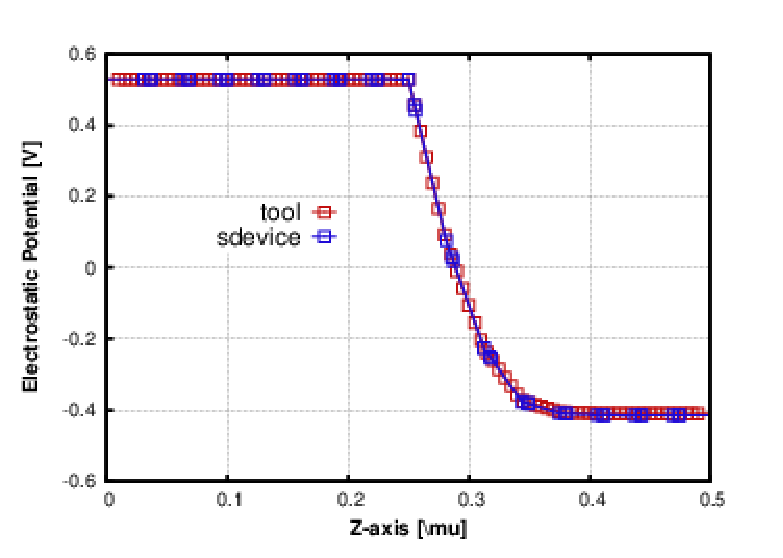
\includegraphics[scale=0.3]{N1e19_P1e17}}
	\subfigure[N20P20]
	  {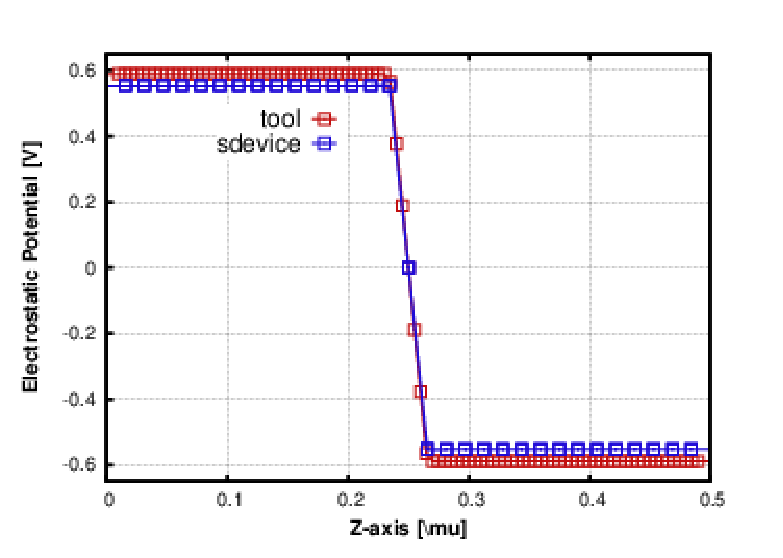
\includegraphics[scale=0.3]{N1e20_P1e20_block_POT_Z}}
\end{figure}
\end{center}
\end{column}
\begin{column}{0.5 \textwidth}
\begin{center}
\begin{figure}[!h]
         \subfigure[N20P17N19]
          {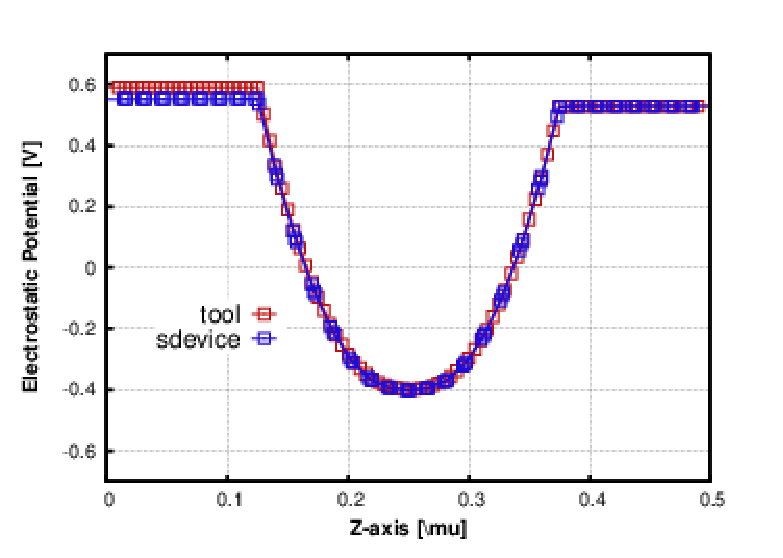
\includegraphics[scale=0.3]{N1e20_P1e17_N1e19}}
	\subfigure[N18P18]
	  {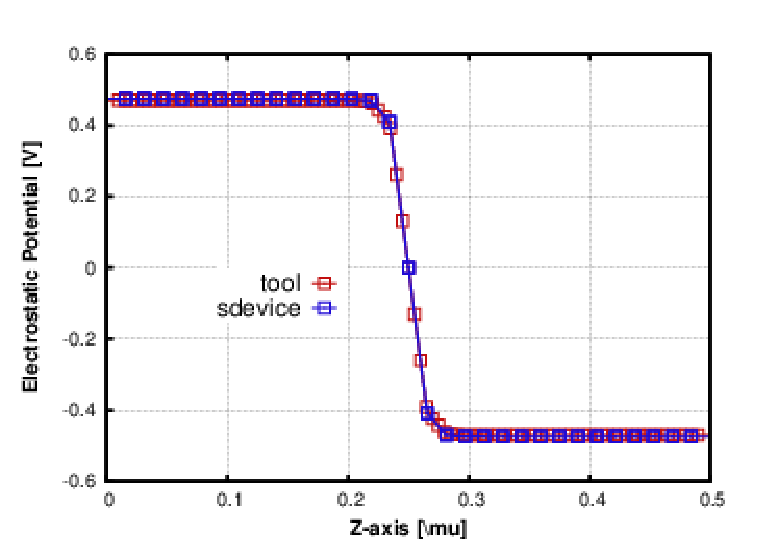
\includegraphics[scale=0.3]{N1e18_P1e18_block_POT}}
\end{figure}
\end{center}
\end{column}
\end{columns}

\end{frame}

\begin{frame}
\frametitle{Free charge plot asse Z \& Newton method (start-end)}
L'accordo si mantiene ottimo al variare della mesh (abbiamo prodotto i test lavorando con mesh fra i 450 a 70.000 nodi). Effettuando tagli ortogonali all'asse Z l'accordo si mantiene ottimo.

\begin{columns}

\begin{column}{0.5 \textwidth}
\begin{figure}[!h]
\subfigure[N18P18]
	  {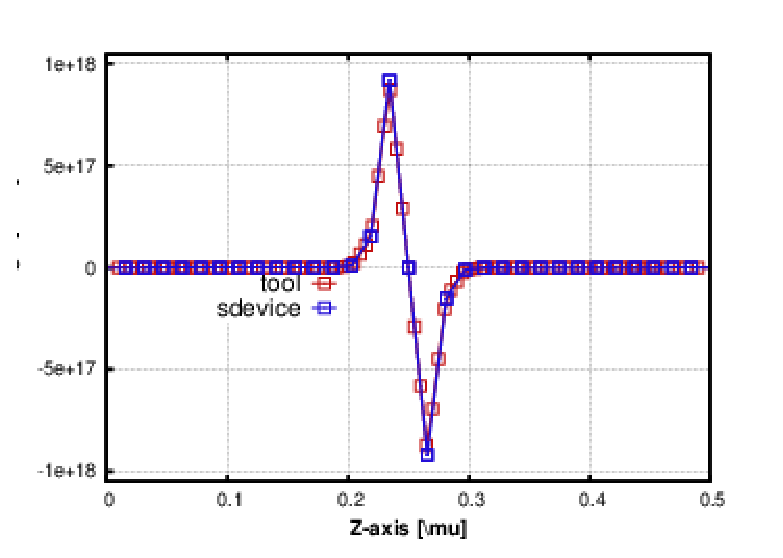
\includegraphics[scale=0.3]{N1e18_P1e18_block_CHARGE}}
	  \end{figure}
\end{column}

\begin{column}{0.5 \textwidth}
\begin{figure}[!h]
	  \subfigure[N20P20]
	  {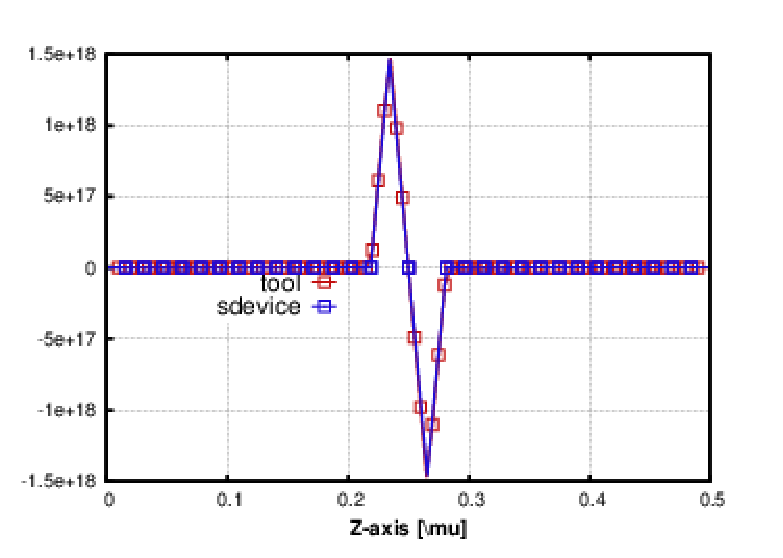
\includegraphics[scale=0.3]{N1e20_P1e20_block_CHARGE_Z}}
	  \end{figure}
\end{column}

\end{columns}

\end{frame}

\begin{frame}
\frametitle{Newton method (start-end) \& Band Diagram}
Per la visualizzazione il livello 0 \`e il vuoto, mentre la risoluzione viene calcolata mettendo a 0 il potenziale di fermi.
\begin{columns}

\begin{column}{0.25 \textwidth}
\begin{center}
\begin{figure}[!h]
          {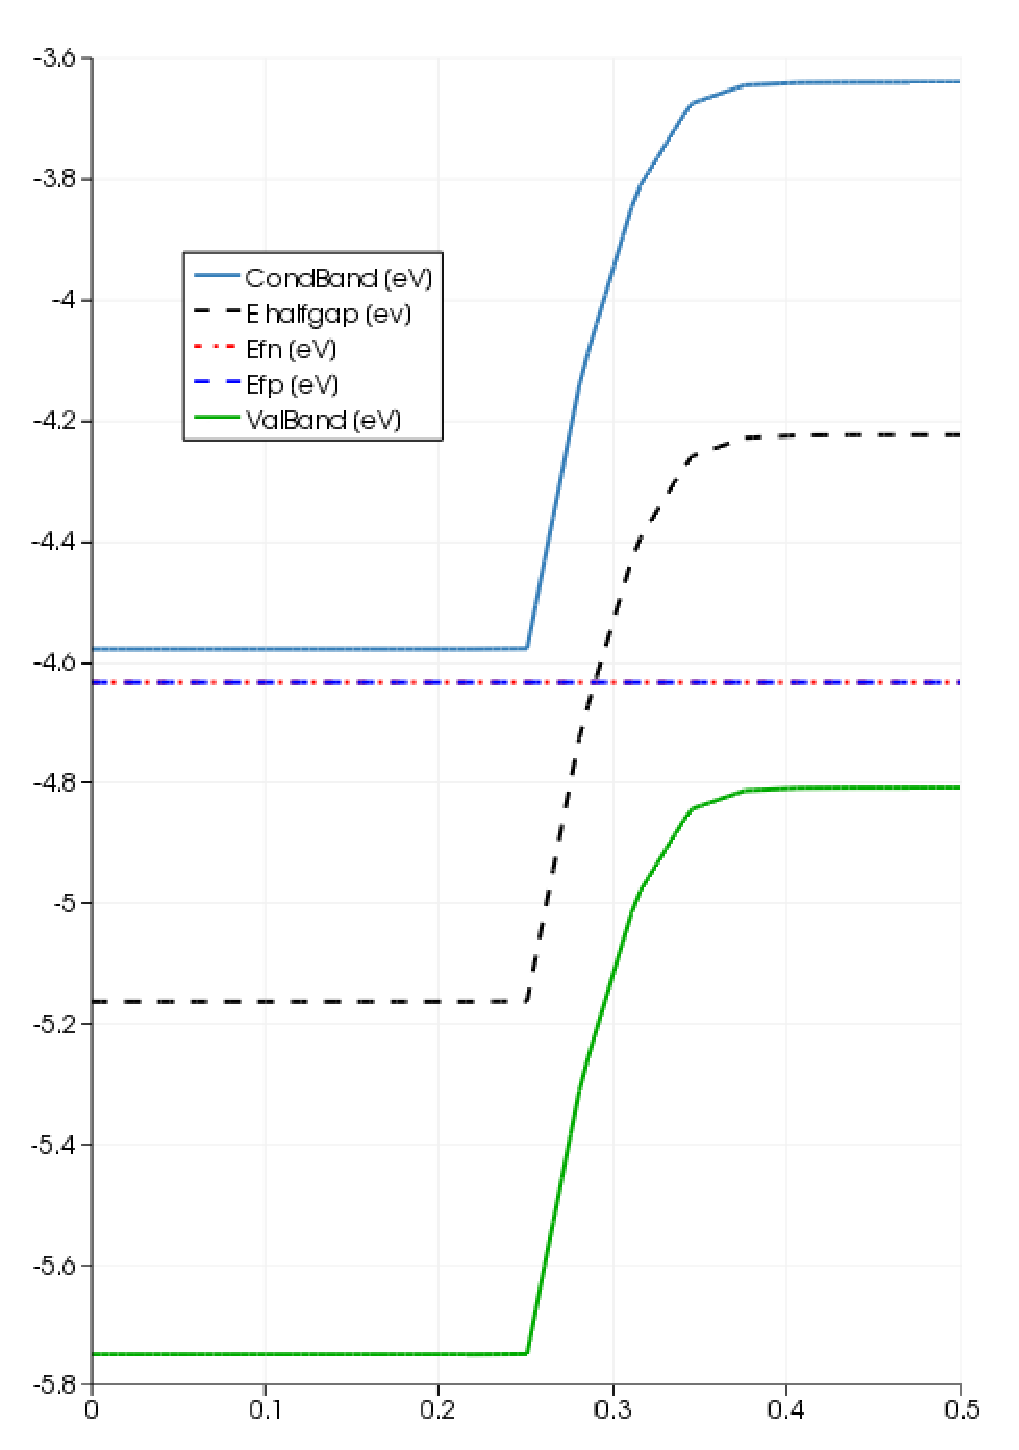
\includegraphics[scale=0.18]{N1e19_P1e17_BandDiagram}}
\end{figure}
\end{center}
\end{column}

\begin{column}{0.25 \textwidth}
\begin{center}
\begin{figure}[!h]
          {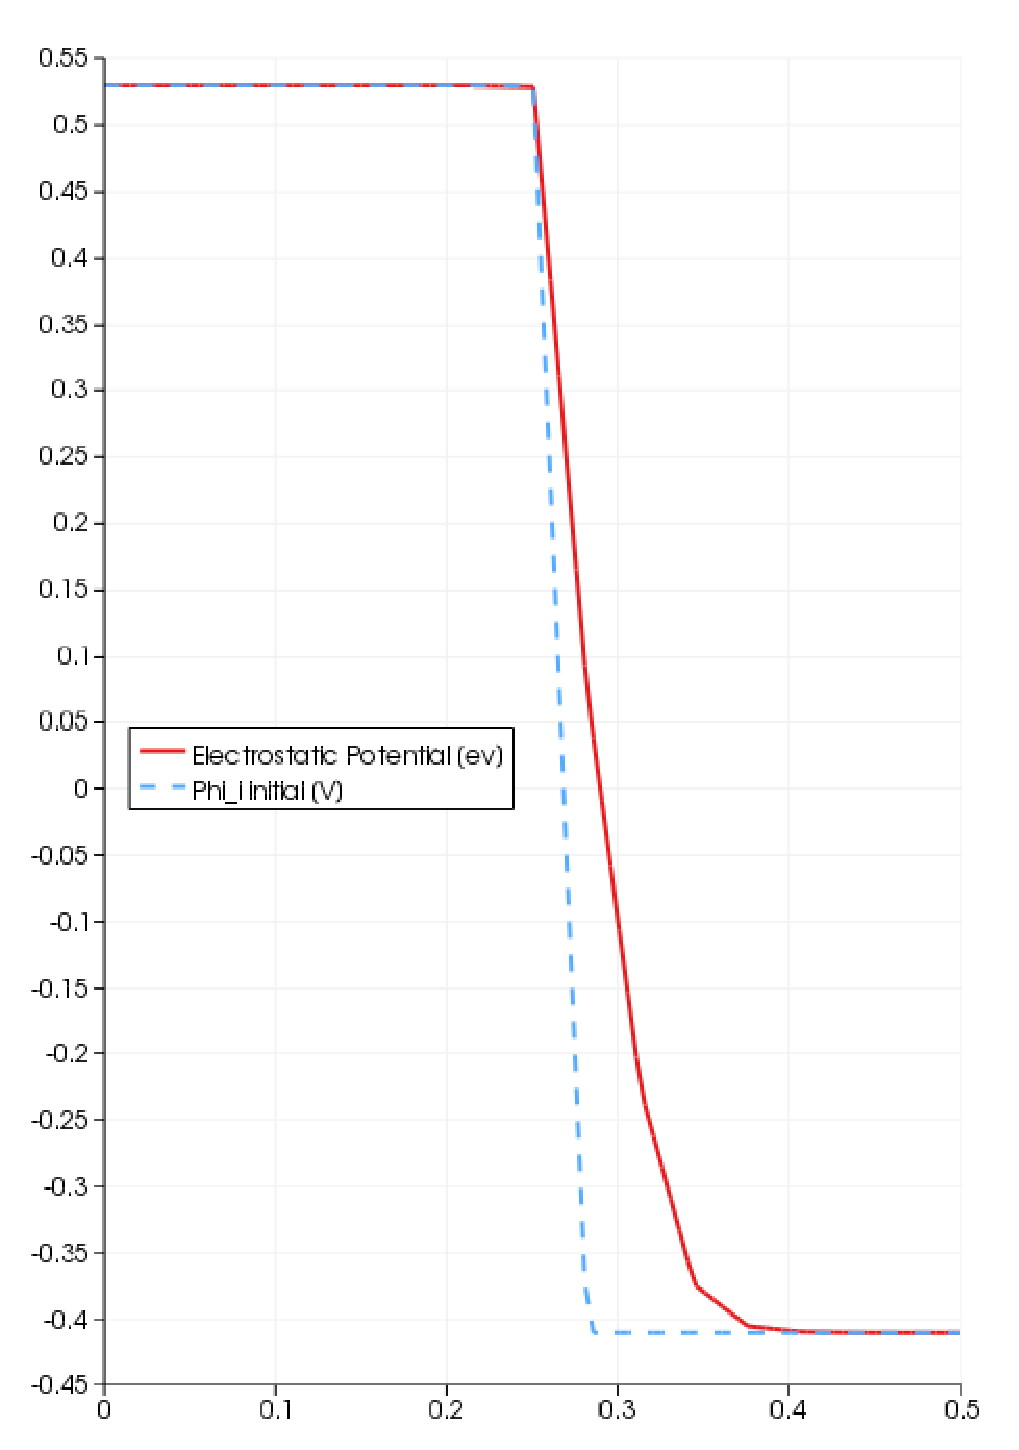
\includegraphics[scale=0.18]{N1e19_P1e17_ElectrostaticPotential}}	
\end{figure}
\end{center}
\end{column}

\begin{column}{0.25 \textwidth}
\begin{center}
\begin{figure}[!h]

          {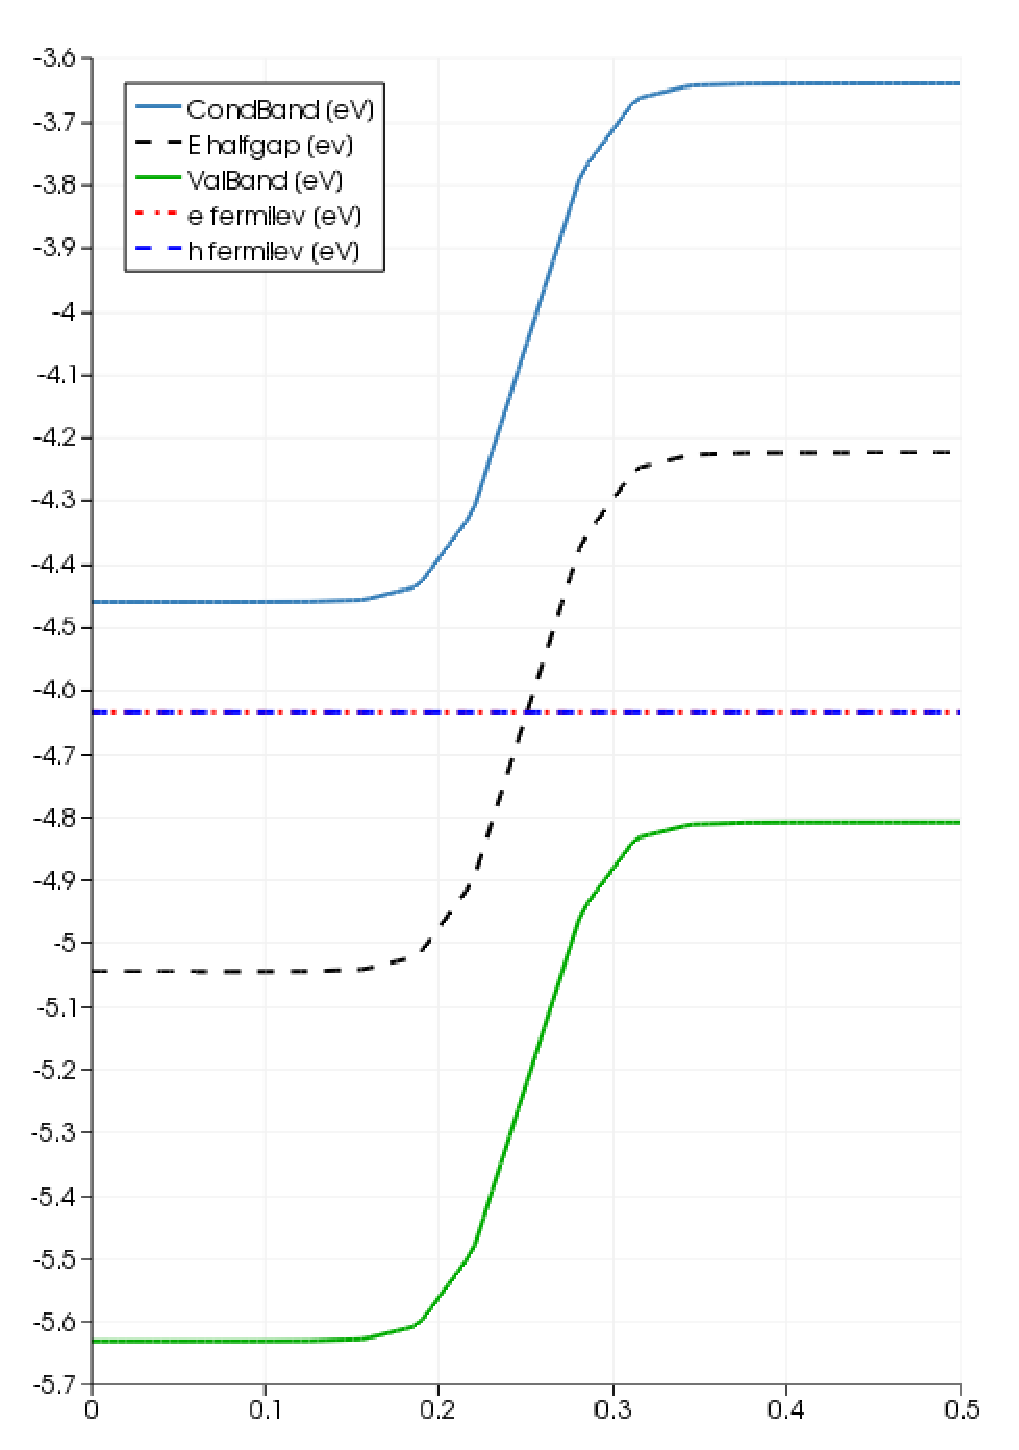
\includegraphics[scale=0.18]{N1e17_P1e17_BandDiagram}}
 \end{figure}
 \end{center}
 \end{column}
 
\begin{column}{0.25 \textwidth}
\begin{center}
\begin{figure}[!h]
          {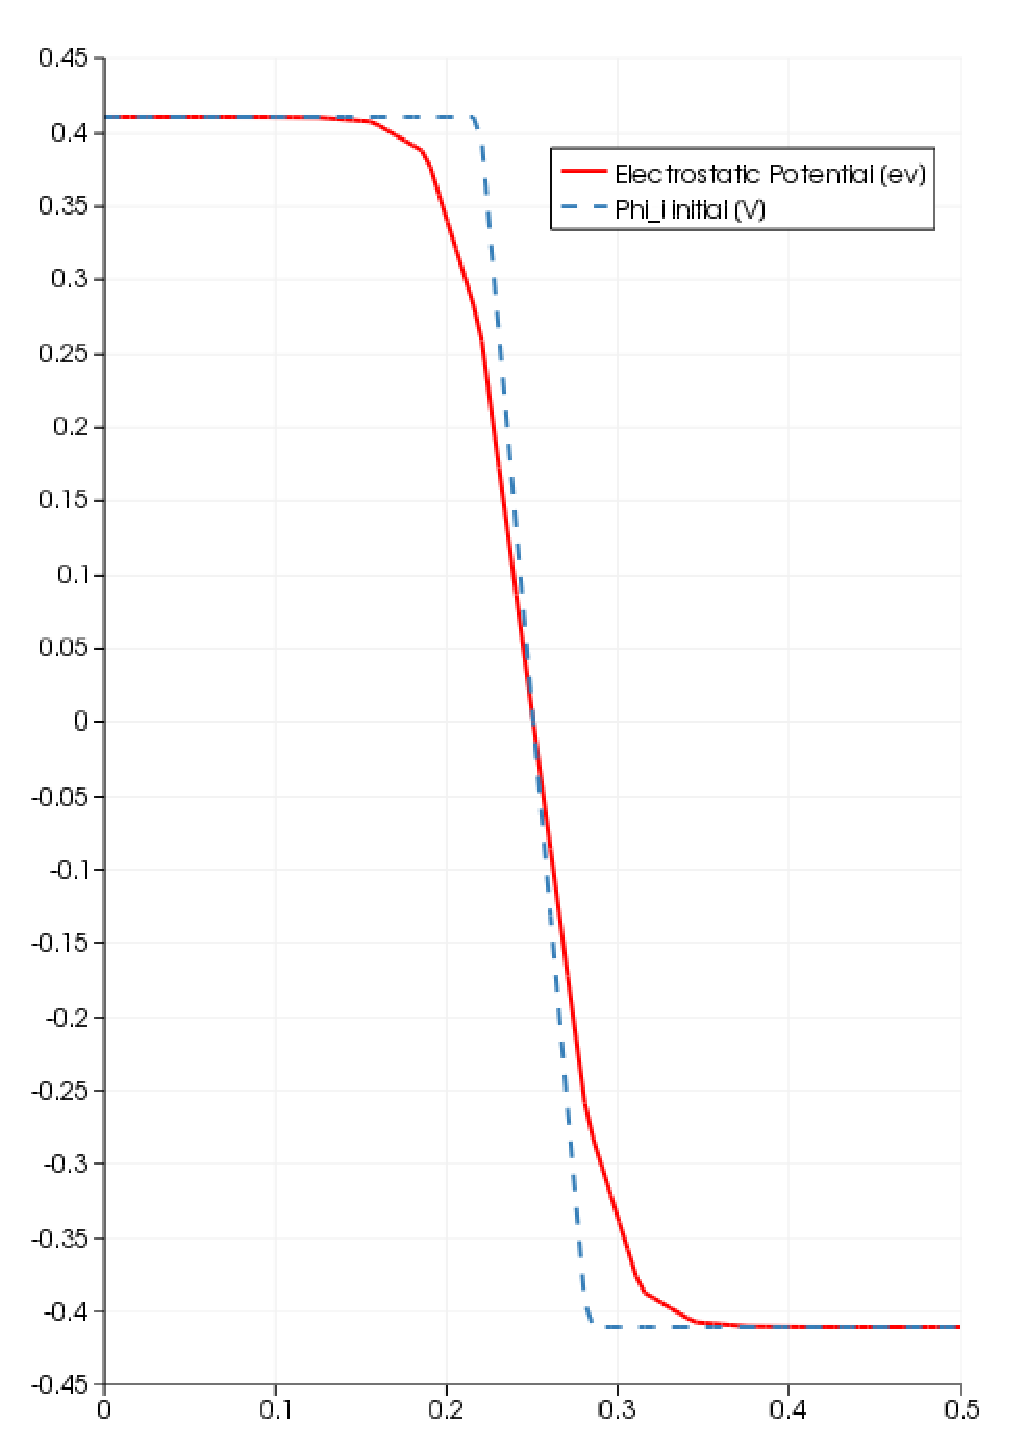
\includegraphics[scale=0.18]{N1e17_P1e17_ElectrostaticPotential}}	
\end{figure}
\end{center}
\end{column}

\end{columns}

\end{frame}



